\label{section:azure}
Moving the analytical back-end to the cloud requires choosing a cloud service provider.\\
Axpo and Reply concorded on relying on {Microsoft Azure Cloud Computing Platform \& Services}.

This chapter will provide a description of the main cloud technologies used for the project.

\section{Introduction}

Microsoft Azure is a cloud computing platform offering several services created by Microsoft.
Many different programming languages, tools and frameworks, including both Microsoft-specific and third-party software and systems are supported\cite{bib:azure:wikipedia}.

Tools, called \textit{Resources} can be organized under a \textit{Resource Group}, a sort of ``container'' which allows to set configurations (e.g. permissions) at a global level.

In this chapter we will analyze the most important tools used for the ETL and analysis processes under the \textit{ToyCase} enviroment.
We will also provide a description of the various environments used.

Figure \ref{fig:azure_resources} shows all resources available in the \textit{ToyCase} environment.

\begin{figure}
    \centering
    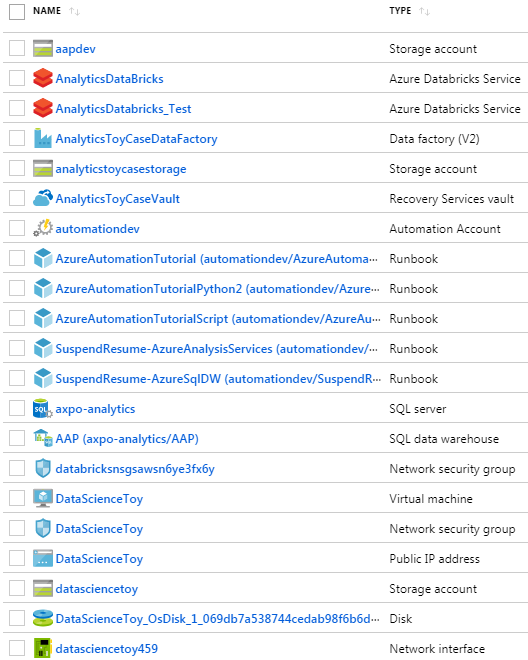
\includegraphics[width=.7\textwidth]{res/azure/toycase.png}
    \caption{Microsoft Azure \textit{ToyCase} Environment Resources.}
    \label{fig:azure_resources}
\end{figure}

\section{Enviroments}
    We define as \textit{environment} a \texttt{resource group}, i.e. a collection of resources that can be managed together.

We created two environments in order to answer to the different needs of the project.
These environment are used respectively for development and production.

All environments have the same tools and configuration, the only difference is how they are used.

\paragraph{Development}
    The development environment, nicknamed \textit{Toycase}, is where Reply develops new functionalities.
    
    This environment may contain work-in-progress scripts, along with some tests on functionalities or data.
    Moreover, the data warehouse contains only a portion of the data needed by the algorithms, since the purpose of this environment is to test whether the downloader works.
    
\paragraph{Production}
    The production environment is architecturally identical to the development environment, but it is actively used by end-users and their algorithms.
    
    This environment contains up to several years of data history for each provider and constantly downloads new information when scheduled.
    
    All the code on this environment must always work without errors.
    To guarantee this, all the code has to be previously tested on the development environment.



\section{Resources}
    This section will describe the main Azure resources used for downloading, storing and processing the data.
    \subsection{Databricks}
        \label{section:azure:databricks}

\textit{Azure Databricks} is an Apache Spark-based analytics platform optimized for the Microsoft Azure cloud services platform \cite{bib:azure:databricks:description}.

Databricks allows full management of Spark clusters, along with online editing of scripts, which are used to create and submit jobs to the cluster.

\subsubsection{Folder structure}
    Databricks provides a single workspace shared across all users.
    It is possible to create and manage folders and files under this workspace.
    
    By default, there are two folders with special permissions already set-up.
    
    \paragraph{Shared}
        All objects stored under the \texttt{Shared} folder are public, meaning that all users have read, write and execute permissions on them.
        
        This folder can be used as a quick way to share items between users, especially if they have different or incompatible permissions.
        
    \paragraph{Users}
        The \texttt{Users} folder contains a subfolder for each user who has access to Databricks.
        
        By default, each user is the administrator of their own folder, but they can also give permissions to other users.

\subsubsection{Coding}
    Databricks allows programming in the following languages:
        \begin{itemize}
            \item Python
            \item Scala
            \item R
            \item SQL
            \item Bash
        \end{itemize}
    
    Scripts are divided into several cells, similarly to a Python notebook.
    
    Each cell must be written in a single programming language, but a script can contain cells in different languages.
    
    In order to specify how a script should be interpreted it is sufficient to write the language used in the first line of the cell.
    
    Figures \ref{fig:azure:databricks:scala}, \ref{fig:azure:databricks:python} and \ref{fig:azure:databricks:bash} show a cell in Scala, one in Python, and one in Bash, respectively.
    These different cells can even belong to the same script.

    \begin{figure}
        \centering
        \begin{subfigure}{0.4\textwidth}
            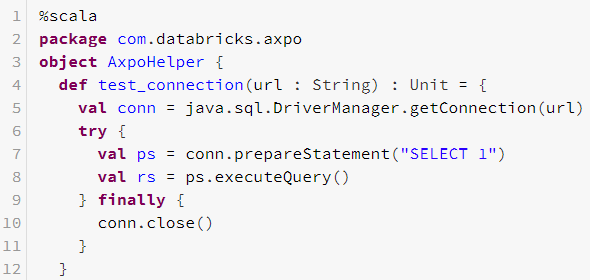
\includegraphics[width=\textwidth]{res/azure/databricks/scala.png}
            \subcaption{Scala}
            \label{fig:azure:databricks:scala}
        \end{subfigure}
        
        \begin{subfigure}{0.4\textwidth}
            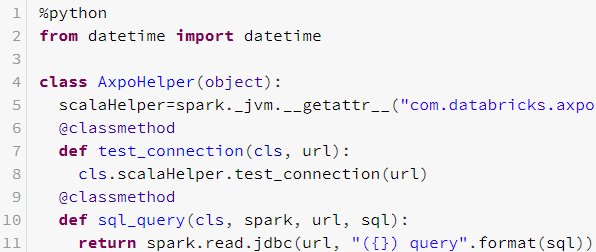
\includegraphics[width=\textwidth]{res/azure/databricks/python.png}
            \subcaption{Python}
            \label{fig:azure:databricks:python}
        \end{subfigure}
        
        \begin{subfigure}{0.4\textwidth}
            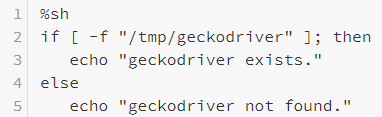
\includegraphics[width=\textwidth]{res/azure/databricks/bash.png}
            \subcaption{Bash}
            \label{fig:azure:databricks:bash}
        \end{subfigure}
        
        \caption{Different scripting languages in Databricks.}
    \end{figure}
    
\subsubsection{Permissions}
    Admins can specify advanced permissions for each folder or even file.
    
    It is possible to assign permissions to both single users and groups.
    
    Figure \ref{fig:azure:databricks:permissions} shows an example of permissions, which are set on a folder called ETL.
    All users belonging the the group ``admins'' can manage the folder and its content, while the user ``Mario P***'' can only read its content.
    
    \begin{figure}
        \centering
        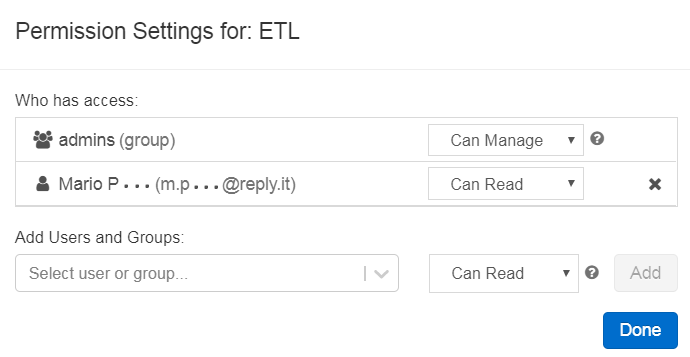
\includegraphics[width=.7\textwidth]{res/azure/databricks/permissions.png}
        \caption{Azure Databricks folder permissions.}
        \label{fig:azure:databricks:permissions}
    \end{figure}
    
    \paragraph{Options}
        There are different permission options.
        These are:
        \begin{enumerate}
            \item No permissions
                \begin{itemize}
                    \item Users cannot do anything with this object
                \end{itemize}
            \item Can Read
                \begin{itemize}
                    \item Users can read and comment notebooks in the folder
                \end{itemize}
            \item Can Run
                \begin{itemize}
                    \item Users can read, comment, attach/detach and run commands in notebooks in the folder
                \end{itemize}
            \item Can Edit
                \begin{itemize}
                    \item In addition to the above, users can also modify notebooks in the folder
                \end{itemize}
            \item Can Manage
                \begin{itemize}
                    \item Users can do all of the above, as well as assign permissions to others
                \end{itemize}
        \end{enumerate}
        
    \paragraph{Groups}
        Permissions can also be assigned at group-level.
        Groups are a collection of users which share the same permissions.
        
        A default group, called ``admins'' has manage permissions on all objects in Databricks.
        Other groups can be freely created and managed.
        
    \paragraph{Default permissions}
        By default, admins have \textit{manage} permissions on all items in Databricks.
        They have full access to any file, which means that they can also see proprietary algorithms or other company secrets.
        
        Each user has also \textit{manage} permissions on their personal folder, under the directory ``Users''.
        This place acts as their personal workspace, in which they can perform any action.
        
        There is also a shared folder in which all users have by default all permissions.
        This folder is useful as a quick way of sharing code between users, especially if they have different permissions, or if they want to share only specific files.

\subsubsection{Execution}
    All scripts create a job identified by an UUID\footnote{Universally Unique Identifier}.
    These jobs are executed on an Apache Spark cluster.
    
    All standard operations of a cluster are available, such as viewing running, queued and completed jobs, inspecting job stages and inspecting and changing cluster configuration.
    
    All of these options can be selected through a standard SparkUI interface, such as the one shown in Figure \ref{fig:azure:databricks:sparkui}.
    
    \begin{figure}
        \centering
        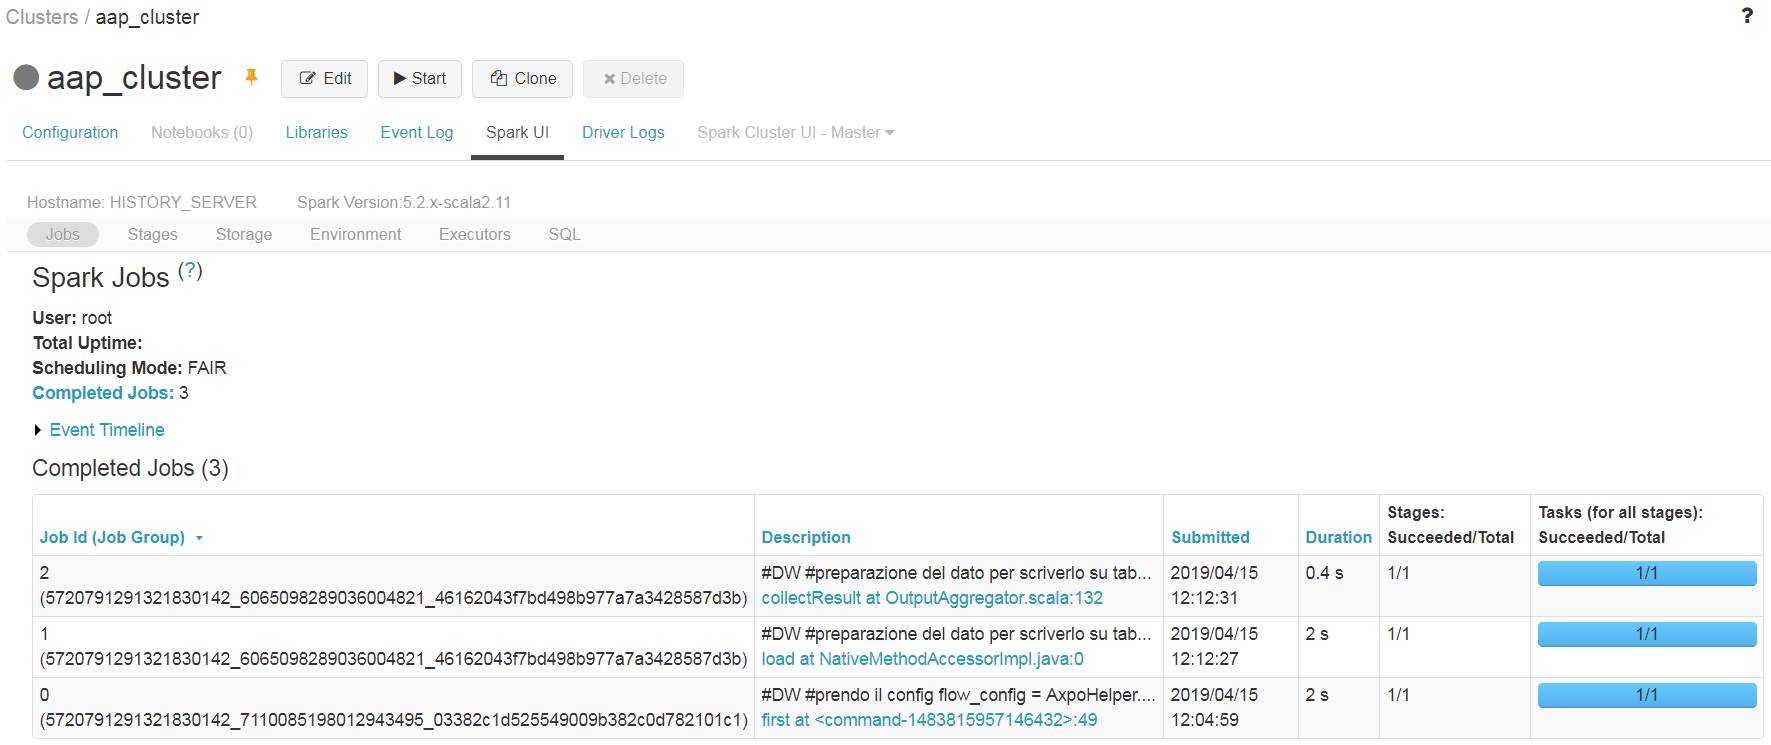
\includegraphics[width=\textwidth]{res/azure/databricks/sparkui.png}
        \caption{Databricks SparkUI interface.}
        \label{fig:azure:databricks:sparkui}
    \end{figure}
    
    \paragraph{Cluster specifications}
        The cluster is composed of two nodes: one is both master and worker, the other serves only as worker.
        Each node has 14 GB RAM available and 4 cores.
        
        One of the most important aspects of Databricks is called \textit{autoscaling}.
        If the cluster is currently executing a computationally demanding task, Databricks may choose to add some workers to increase performance.
        It is possible to set both the minimum and the maximum amount of workers.

        Autoscaling is useful when facing variable loads, since it allows to save up some costs by shutting off some workers that are not needed, whereas in a statically-sized cluster all workers would be constantly active.
        
\subsubsection{Importing/Exporting scripts}
    Databricks allows exporting and importing scripts by directly interacting with the user interface, from which it is possible to export a whole folder in \texttt{zip} format.
    Similarly, it is also possible to import a zipped folder into a different environment.
    Alternatively, a single file can also be directly exported in their native format.

    \subsection{DataLake}
        \label{section:azure:datalake}
\label{todo:datalake_description}
\textit{Azure DataLake Gen2} is a cloud storage service.
It is possible to store and retrieve files of any format and up to 8TB size.

\subsubsection{Blob storage}
    Files are stored under a Blob storage format, which is an Azure-developed format optimized for storing massive amounts of unstructured data \cite{bib:azure:datalake:intro_to_blob_storage}.
    
    Blob storage offers three types of resources:
        \begin{itemize}
            \item The storage account.
            \item A container in the storage account.
            \item A blob in a container.
        \end{itemize}

    Figure \ref{fig:azure:datalake:resources_relationship} shows the relationship between these resources.
    Files are memorized in a blob, i.e, a particular distributed storage format which can contain pieces of multiple files.
    
    \begin{figure}
        \centering
        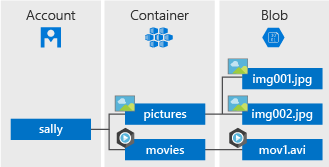
\includegraphics[width=.5\textwidth]{res/azure/datalake/blob.png}
        \caption{Relationship between DataLake resources.}
        \label{fig:azure:datalake:resources_relationship}
    \end{figure}

    Permissions can be set at container level or at file level.
    Under each container it is possible to upload or download files, or to organize them into sub-folders.
    
    Data can be accessed through HTTP or HTTPS.
    It is also possible to mount the Blob storage as a file system through the \texttt{abfss}\footnote{
        \textit{Azure Blob File System}. The last \texttt{s} means the protocol is \textit{Secure}, i.e., it requires SSL authentication.
    } protocol.
    \paragraph{Blob types}
        Azure Storage supports three types of blobs \cite{bib:azure:datalake:intro_to_blob_storage}:
            \begin{itemize}
                \item Block blobs store text and binary data, up to about 4.7 TB. Block blobs are made up of blocks of data that can be managed individually.
                \item Append blobs are made up of blocks like block blobs, but are optimized for append operations. Append blobs are ideal for scenarios such as logging data from virtual machines.
                \item Page blobs store random access files up to 8 TB in size. Page blobs that store the virtual hard drive files serve as disks for Azure virtual machines.
            \end{itemize}
            
        All files used by Databricks, given their relatively small size (a few MB per file) are stored as block blobs.


    \subsection{SQL Data Warehouse}
        Azure SQL Data Warehouse is a cloud-based data warehouse that uses Massive Parallel Processing (MPP).

MPP allows a high number of processors, even located on different machines, to work on different parts of the same task simultaneously.

Thanks to MPP it is possible to run complex queries across petabytes of data.

\subsubsection{Data storage}
    The data warehouse data is stored separately on Azure Storage.
    
    The data itself is sharded into several \textbf{distributions} across different nodes, to improve performance.

\subsubsection{Massive Parallel Processing}
    Massive Parallel Processing is managed in Azure SQL Data Warehouse by a node-based architecture \cite{bib:azure:dwh:mpp}, as shown in Figure \ref{fig:azure:dwh:mpp}.
    
    \begin{figure}
        \centering
        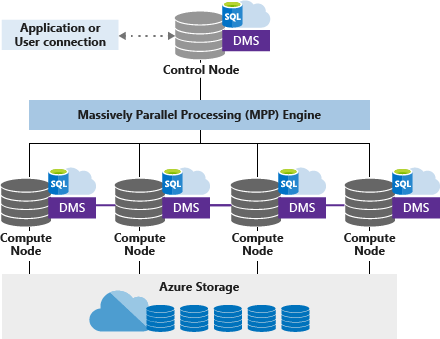
\includegraphics[width=.6\textwidth]{res/azure/dwh/mpp.png}
        \caption{Azure SQL Data Warehouse MPP architecture.}
        \label{fig:azure:dwh:mpp}
    \end{figure}
    
    Queries are sent to the Control node, which optimizes the work for parallel processing, before sending it to Compute nodes, which execute it.
    
    \paragraph{Control node}
        The control node can be defined as the brain of the data warehouse.
        It receives commands and runs a MPP engine, which optimizes and coordinates the work.
        
        Queries are split into 60 smaller queries\footnote{
            This value appears to be fixed and independent from which the query executed \cite{bib:azure:dwh:mpp}.
        } which can all be run in parallel.
        
        The smaller queries are then assigned to a number of Compute nodes, which execute them.
        
        Each smaller query is executed on a single data distribution.
        
    \paragraph{Compute nodes}
        A compute node is a working unit which executes queries received by the Control node.
        
        An Azure SQL Data Warehouse can have up to 60 compute nodes.
        Depending on how many nodes are available to the system\footnote{
            Their number depends on the chosen plan tier. A higher number of compute nodes comports an higher subscription cost.
        }, the Control node assigns them from 1 to 60 distributions.
        
        For example, if there are 60 nodes available each one will have to compute a single task, whereas if only a single node is available it will have to execute all 60 tasks.

\subsubsection{Limitations}
    MPP allows a low number of parallel queries, which are a fundamental requirement, given that several users will be working the data warehouse at the same time.
    
    Azure SQL data warehouse offers different capacity plan, with different costs and computational power.
    The plan currently chosen by Reply allows up to 12 queries in parallel, which, although is enough for development, it is much too low for the actual needs of the trading and big data departments combined.
    
    The highest plan tier offers up to 128 queries in parallel at more than ten times the actual cost \cite{bib:azure:databricks:concurrency_limits}.
    Even ignoring the economic effects of this choice, the number of queries offered is still not high enough, which means that the data warehouse might not be able to answer all queries in acceptable times.
    
    The solution to this problem is to create a replica of a portion of the data warehouse and to perform the most computationally demanding queries there.
    These replicas will reside on Azure Analysis Services.
    
    \subsection{PolyBase}
        PolyBase is a tool which allows the SQL Data Warehouse to process SQL queries on data from external sources \cite{bib:azure:polybase}.

The most common external source is Azure Blob Storage.
PolyBase is able to create a connection layer between the Data Warehouse and Blob files.
These files appear to the user as normal external tables.
These files can then be directly queried through SQL.

PolyBase is natively available on Microsoft Azure, so there's no need to perform a manual installation.
The tool is also often transparent to the users, so most times it is actually used without even realizing it.

PolyBase relies on Hadoop to perform cross-source SQL operations.

\paragraph{Advantages}
    Without PolyBase, querying a SQL Data Warehouse along with an external source would require either transferring half of the data available, bringing all data in a single format, or performing two separate queries and writing custom client-side logic to join the data obtained.
    
    With PolyBase this problem is removed, since users can directly query both sources at once using SQL, without having to transfer anything beforehand.

\paragraph{Performance}
    PolyBase can push computation to Hadoop to improve performance.
    The decision is handled by PolyBase's own query optimizer, which uses statistics on external tables to make the cost-based decision.
    Computations on Hadoop create MapReduce jobs which leverage distributed computational resources.
    \subsection{Other resources}
        \subsubsection{Data Factory}
            Azure Data Factory can be defines as a cloud-based data integration service that allows users to create data-driven workflows in the cloud for orchestrating and automating data movement and data transformation \cite{bib:azure:datafactory:intro}.

Users can create workflows that ingest data from different sources.
These workflows can apply operation of the data using different cloud services, such as Hadoop or Spark.
The results can be published to cloud data stores, such as Azure SQL Data Warehouse or Azure Data Lake.

\paragraph{Advantages and Limitations}
    This service is very effective for performing basic operations, such as reading from a data source and writing on a different one.
    Basic transformation operations can also be applied.
    
    These simple workflows can be developed in just a few minutes using the graphical interface.
    
    However, this tool isn't suited for more complex operations, since it isn't possible to write code directly, but it is necessary to use the user interface.
    In these cases, coding in Databricks proves to be easier and more versatile.
        \subsubsection{Virtual Machine}
            A virtual machine can be run on the Azure cloud services.

The machines can be customized depending on the user needs, with options ranging from the operating system to vCPUs\footnote{
    \textit{Virtual CPU}.
    A vCPU is a share of a physical CPU that is assigned to a virtual machine.
    It is possible to assign multiple \textit{vCPUs} to a single Azure Virtual Machine.
} and RAM available.

The chosen virtual machine runs Windows Server, with a graphical environment installed.

Users can install their own applications on the machine, running code in languages or environments not supported by Azure Databricks.
        \subsubsection{Analysis Services}
            Azure Analysis Services allows users to combine and analyze data from multiple sources.

Users can apply operations or filters on data sources, as well as display the results in multiple graphical formats, such as maps, charts or reports.

This service has not been used during development, but will be used once the entire migration process will be completed to perform Business Intelligence analysis on the data contained in the data warehouse.
        \subsubsection{Automation Account}
            Azure Automation Account allows user to schedule management operations for the whole environment.

Users can create \textit{Runbooks}, which are a set of scheduled commands, and execute them.

Runbooks can be created either through a graphical interface or by using Python or Powershell.

A single runbook can contain multiple jobs, each one performing a single task.
Each job can be scheduled to be executed at a specific time.


    
